% Copyright (c) 2008-2009 solvethis
% Copyright (c) 2010-2016 Casper Ti. Vector
% Public domain.
%
% 使用前请先仔细阅读 pkuthss 和 biblatex-caspervector 的文档,
% 特别是其中的 FAQ 部分和用红色强调的部分。
% 两者可在终端/命令提示符中用
%   texdoc pkuthss
%   texdoc biblatex-caspervector
% 调出。

% 采用了自定义的(包括大小写不同于原文件的)字体文件名,
% 并改动 ctex.cfg 等配置文件的用户请自行加入 nofonts 选项;
% 其它用户不用加入 nofonts 选项,加入之后反而会产生错误。
\documentclass[UTF8]{pkuthss}

% 使用 biblatex 排版参考文献,并规定其格式(详见 biblatex-caspervector 的文档)。
% 这里按照英文文献在前,中文文献在后排序(“sorting = ecnty”);
% 若需按照中文文献在前,英文文献在后排序,请设置“sorting = centy”;
% 若需按照引用顺序排序,请设置“sorting = none”。
% 若需在排序中实现更复杂的需求,请参考 biblatex-caspervector 的文档。
\usepackage[backend = biber, style = caspervector, utf8, sorting = ecnty]{biblatex}

% 代码
\usepackage{listings}
\usepackage{color}

\definecolor{dkgreen}{rgb}{0,0.6,0}
\definecolor{gray}{rgb}{0.5,0.5,0.5}
\definecolor{mauve}{rgb}{0.58,0,0.82}
\lstset{ %
  language=Octave,                % the language of the code
  basicstyle=\footnotesize,           % the size of the fonts that are used for the code
  numbers=left,                   % where to put the line-numbers
  numberstyle=\tiny\color{gray},  % the style that is used for the line-numbers
  stepnumber=2,                   % the step between two line-numbers. If it's 1, each line 
                                  % will be numbered
  numbersep=5pt,                  % how far the line-numbers are from the code
  backgroundcolor=\color{white},      % choose the background color. You must add \usepackage{color}
  showspaces=false,               % show spaces adding particular underscores
  showstringspaces=false,         % underline spaces within strings
  showtabs=false,                 % show tabs within strings adding particular underscores
  frame=single,                   % adds a frame around the code
  rulecolor=\color{black},        % if not set, the frame-color may be changed on line-breaks within not-black text (e.g. commens (green here))
  tabsize=2,                      % sets default tabsize to 2 spaces
  captionpos=b,                   % sets the caption-position to bottom
  breaklines=true,                % sets automatic line breaking
  breakatwhitespace=false,        % sets if automatic breaks should only happen at whitespace
  title=\lstname,                   % show the filename of files included with \lstinputlisting;
                                  % also try caption instead of title
  keywordstyle=\color{blue},          % keyword style
  commentstyle=\color{dkgreen},       % comment style
  stringstyle=\color{mauve},         % string literal style
  escapeinside={\%*}{*)},            % if you want to add LaTeX within your code
  morekeywords={*,...}               % if you want to add more keywords to the set
}

% 按学校要求设定参考文献列表中的条目之内及之间的距离。
\setlength{\bibitemsep}{3bp}
% 对于 linespread 值的计算过程有兴趣的同学可以参考 pkuthss.cls。
\renewcommand*{\bibfont}{\zihao{5}\linespread{1.27}\selectfont}

% 设定文档的基本信息。
\pkuthssinfo{
	cthesisname = {硕士研究生学位论文}, ethesisname = {Master Thesis},
	ctitle = {基于区块链的PKI实体鉴权方案设计与实现}, etitle = {Test Document},
	cauthor = {李安然},
	eauthor = {Anran Li},
	studentid = {1501214389},
	date = {X年X月},
	school = {信息科学技术学院},
	cmajor = {计算机软件与理论}, emajor = {Software and Theory of Computer},
	direction = {网络与信息安全},
	cmentor = {关志 副研究员}, ementor = {Prof.\ Zhi\.Guan},
	ckeywords = {PKI技术,区块链,身份认证,密码学}, ekeywords = {First, Second}
}
% 载入参考文献数据库(注意不要省略“.bib”)。
\addbibresource{thesis.bib}

% 普通用户可删除此段,并相应地删除 chap/*.tex 中的
% “\pkuthssffaq % 中文测试文字。”一行。
\usepackage{color}
\def\pkuthssffaq{%
	\emph{\textcolor{red}{pkuthss 文档模版最常见问题:}}

	\texttt{\string\cite}、\texttt{\string\parencite} %
	和 \texttt{\string\supercite} 三个命令分别产生%
	未格式化的、带方括号的和上标且带方括号的引用标记:%
	\cite{test-en},\parencite{test-zh}、\supercite{test-en, test-zh}。

	若要避免章末空白页,请在调用 pkuthss 文档类时加入 \texttt{openany} 选项。

	如果编译时不出参考文献,
	请参考 \texttt{texdoc pkuthss}“问题及其解决”一章
	“其它可能存在的问题”一节中关于 biber 的说明。
}

\begin{document}
	% 以下为正文之前的部分,默认不进行章节编号。
	\frontmatter
	% 此后到下一 \pagestyle 命令之前不排版页眉或页脚。
	\pagestyle{empty}
	% 自动生成封面。
	\maketitle
	% 版权声明。封面要求单面打印,故需新开右页。
	\cleardoublepage
	% Copyright (c) 2008-2009 solvethis
% Copyright (c) 2010-2017 Casper Ti. Vector
% All rights reserved.
%
% Redistribution and use in source and binary forms, with or without
% modification, are permitted provided that the following conditions are
% met:
%
% * Redistributions of source code must retain the above copyright notice,
%   this list of conditions and the following disclaimer.
% * Redistributions in binary form must reproduce the above copyright
%   notice, this list of conditions and the following disclaimer in the
%   documentation and/or other materials provided with the distribution.
% * Neither the name of Peking University nor the names of its contributors
%   may be used to endorse or promote products derived from this software
%   without specific prior written permission.
%
% THIS SOFTWARE IS PROVIDED BY THE COPYRIGHT HOLDERS AND CONTRIBUTORS "AS
% IS" AND ANY EXPRESS OR IMPLIED WARRANTIES, INCLUDING, BUT NOT LIMITED TO,
% THE IMPLIED WARRANTIES OF MERCHANTABILITY AND FITNESS FOR A PARTICULAR
% PURPOSE ARE DISCLAIMED. IN NO EVENT SHALL THE COPYRIGHT HOLDER OR
% CONTRIBUTORS BE LIABLE FOR ANY DIRECT, INDIRECT, INCIDENTAL, SPECIAL,
% EXEMPLARY, OR CONSEQUENTIAL DAMAGES (INCLUDING, BUT NOT LIMITED TO,
% PROCUREMENT OF SUBSTITUTE GOODS OR SERVICES; LOSS OF USE, DATA, OR
% PROFITS; OR BUSINESS INTERRUPTION) HOWEVER CAUSED AND ON ANY THEORY OF
% LIABILITY, WHETHER IN CONTRACT, STRICT LIABILITY, OR TORT (INCLUDING
% NEGLIGENCE OR OTHERWISE) ARISING IN ANY WAY OUT OF THE USE OF THIS
% SOFTWARE, EVEN IF ADVISED OF THE POSSIBILITY OF SUCH DAMAGE.

% 此处不用 \specialchap,因为学校要求目录不包括其自己及其之前的内容。
\chapter*{版权声明}
% 综合学校的书面要求及 Word 模版来看,版权声明页不需加页眉、页脚。
\thispagestyle{empty}

任何收存和保管本论文各种版本的单位和个人,
未经本论文作者同意,不得将本论文转借他人,
亦不得随意复制、抄录、拍照或以任何方式传播。
否则一旦引起有碍作者著作权之问题,将可能承担法律责任。

% 若需排版二维码,请将二维码图片重命名为“barcode”,
% 转为合适的图片格式,并放在当前目录下,然后去掉下面 2 行的注释。
%\vfill\noindent
%\includegraphics[height = 5em]{barcode}

% vim:ts=4:sw=4


	% 此后到下一 \pagestyle 命令之前正常排版页眉和页脚。
	\cleardoublepage
	\pagestyle{plain}
	% 重置页码计数器,用大写罗马数字排版此部分页码。
	\setcounter{page}{0}
	\pagenumbering{Roman}
	% 中英文摘要。
	% Copyright (c) 2014,2016 Casper Ti. Vector
% Public domain.

\begin{cabstract}
	\pkuthssffaq % 中文测试文字
\end{cabstract}

\begin{eabstract}
	Test of the English abstract.
\end{eabstract}

% vim:ts=4:sw=4

	% 自动生成目录。
	\tableofcontents

	% 以下为正文部分,默认要进行章节编号。
	\mainmatter
	% 序言。
	%% Copyright (c) 2014,2016 Casper Ti. Vector
% Public domain.

\specialchap{序言}
\pkuthssffaq % 中文测试文字。

% vim:ts=4:sw=4

	% 各章节。
	% Copyright (c) 2014,2016 Casper Ti. Vector
% Public domain.

\chapter{绪论}

\section{背景知识和研究意义}

随着网路技术的迅猛发展,大量的信息需要通过网络进行交互,在其给人们带来巨大便利的同时,也存在着巨大的安全隐患。在网络中传输的数据可能会被恶意的攻击方非法的窃听,导致传输信息的泄露,如何保证数据在传输过程中的机秘密性、完整性和不可否认性一直是网络安全技术所关注的问题,而公钥基础设施PKI(Public Key Infrastructure)技术是解决这一问题的重要手段.


公钥基础设施PKI作为利用非对称加密算法原理和技术实现并提供安全服务的技术和规范,已经成为互联网中保证数据传输保密性、完整性和不可否认性的重要组成部分。PKI体系中的证书,已经被广泛地应用在各种身份认证的场景下,特别是在互联网中建立SSL通信的过程中,用于保证客户端对服务器身份的认证。


证书在PKI系统中作为公钥和标识绑定的载体,起着流通信任的作用。围绕证书而言,在该系统存在的角色主要包括以下三类:授权机构(CA),用户以及依赖方。在PKI系统中,用户发起证书签发请求,递交给授权机构;授权机构负责证书的签发吊销等管理工作;依赖方则是证书的受用对象,检查证书的合法性并从中获得对方的公钥。

证书是否有效是通过验证该证书是否由授权机构所签发来决定的。依赖方会事先将所有授权机构的相关证书下载到本地,在通信过程中获取对方证书和证书链来验证证书的有效性;而证书附有公钥和标识的绑定关系,之后会用该公钥与对方进行通信,并认为拥有对应私钥的人就是绑定标识者。也就是说,授权机构是整个系统中的信任支点,系统中的依赖方需要对其签发的证书给予绝对信任。如果授权机构有作恶行为,比如签发虚假的证书,网络中的实体并不能辨认该证书的真伪,导致系统中的依赖方与虚假的身份进行通信。

在现有的PKI系统中,授权机构和用户之间的权利是不对等的,用户只能发起证书签发请求,而不能对授权机构是否签发证书起到制约性。由于信任都集中在中心化的授权机构之上,恶意的授权机构或者被攻破的授权机构将可以签发任意用户的证书,从而对相应用户发起中间人攻击,对整个系统带来恶劣的影响。比如在2011年,DigiNotar遭到入侵,签发的虚假证书涉及到20多个网域的200多个SSL证书\supercite{prins2011diginotar},对用户造成了巨大影响,最终导致自身被吊销授权机构资格的后果。

由于授权机构以中心化的形式存在于PKI系统中,并受到了所有实体的绝对信任,一旦其出现问题那么将会瓦解整个信任体系。为了防止授权中心的不端行为,如何去平衡PKI系统中实体的权利一直都是大家说关注的问题。如果授权中心在签发证书前也需要用户同意,那么将会大大减小授权中心被攻破或有不端行为所带来的影响。

区块链作为比特币底层的核心技术,具有去中心化、防篡改的特性,使得比特币与传统货币相比无需信任中心,不依赖第三方来保证其上交易过程的安全性。比特币由于不需要中心化的发行机构,不会被组织或政府操控的特性,受到大家的广泛关注。从最初的类似比特币这样的密码货币争相发布,到现在与区块链相关的传统应用出现在大家的视野中,区块链技术逐渐的被应用在其它领域,其去中心化、防篡改的特性成为了这些应用的核心所在。

如前面所说的那样,PKI中授权中心和用户之间权利不对等,如何去减弱用户对授权中心的依赖十分重要。而区块链技术作为应用在P2P网络中的底层技术,可以在无需中心的情况下,完成对网络中事务的状态统一,保证该网络中实体的各自权益对等。区块链的这些特性可以借鉴并应用到PKI系统中,解决PKI中实体之间的权利不对等所带来的安全隐患,巩固PKI系统的安全。


\section{国内外研究现状}

\subsection{PKI的研究现状}

1976年,美国密码学专家Diffie和Hellman提出了著名的D-H密码分发体制,从而解决了不使用秘密信道进行密钥分发的问题,允许通信双方可以在不安全的通信线路上完成密钥信息交换。在1978年,CA认证中心由Kohnfelder提出,在他给出的方案中,CA集中式的管理公钥,以CA证书的形式公布于目录库中,私钥继续使用秘密信道分发。1996年PKI的解决方案被正式提出,PKI设立CA认证中心,以第三方权威机构的身份完成对公钥和标识的绑定。

经过二十多年的发展,PKI作为提供信息安全服务的基础性普适性设施,无论在理论上还是技术上,都已经日趋成熟。在理论方面,以公钥密码学作为基础的密码算法、协议以及认证方法都得到了全面的发展,为PKI技术提供了安全性保障;在技术上,数字证书的申请、签发和管理,数字证书的相关应用格式,以及PKI实体之的通行协议都被相继提出并制定,使得PKI技术可以按照相应的标准使用在一系列的场景之下。


由于公钥基础设施PKI的存在,我们可以安全地与仅拥有对方公钥的人进行安全通信,通过信任第三方机构CA签发的证书完成公钥与身份的绑定。从安全的角度去审视现有的Internet PKI生态系统,主要存在以下几个方面的问题:首先,最为严重的问题是CA拥有绝对的权利,在未经实体允许的情况下就可以给其签发证书;其次,对CA的信任是没有灵活度的,只存在信任与否的抉择;其三是在域名证书的验证过于薄弱,在传统的方法中只是进过简单的邮箱确认方式,并不是特别安全;最后是证书的吊销不能正常工作,在很多实际使用的情况下,对证书吊销的检查并不完整\supercite{ristic2014bulletproof}。

如上所提及的那样,对CA的信任是绝对的,而且CA拥有绝对有的权利,单个恶意或者被攻破的CA可以给任意一个域名签发证书\supercite{ducklin2013turktrust};同时对于该类假冒的证书,将会需要很大一段时间才能被发现。我们知道全球存在很多很多的CA,不同CA的安全防护能力各不相同,攻击者只需要攻破单个CA,即可签发任意域名的假冒证书,从而对该域名发起中间人攻击,达到攻击相关域名的目的。


%From evaluate web PKI
为了检测通信过程中的证书是否可靠,一些列方案通过依赖方在游览器端询问不同的证书提供者,对比得到的多个证书信息的一致性来确保证书的有效性。Perspectives\supercite{wendlandt2008perspectives}在2008年被Wendlant等人提出,并通过插件的方式应用于FireFox之上,该方案通过在建立安全连接前询问不同的公证服务器来检测该域名的公钥是否合法,一旦发现得到的密钥不相同,将检测出是否有人发起了中间人攻击(MITM)。然而由于证书的传播需要时间,对于新签发的证书可能需要一段时间才可以使用以上的服务,二次验证\supercite{alicherry2009doublecheck}的方案在09年被提出,该方案的主要思路是向目标服务器请求两次证书:一次通过TLS连接,另外一次使用Tor\supercite{alicherry2009doublecheck};该方法在一定程度上同时解决了游览器泄露用户隐私的问题。另外一个Perspectives存在的问题是用户向其请求证书的同时,暴露了自己访问的历史记录,泄露了自身的隐私。为了解决这一问题,Convergence\supercite{convergence}的方案被提出,在用户向公证服务器请求证书的时,将不是直接向某一公证服务器请求数据,而是随机的选择一个公证服务器将其请求转发给其它公证服务器,类似洋葱路由的机制。

由于证书的有效期一般相对比较长,当一个新的证书被使用时,很有可能它是攻击者伪造的证书并发起了攻击,基于这一点Certificate Patrol\supercite{modell2014certificate}的方法在检测到新证书时会向用户发起提示;同时,一般情况下证书的申请也会向自己国家的授权机构发起,当得到一个其它国家的签发的证书时,同样很有可能是虚假的证书,CertLock\supercite{soghoian2011certified}就是基于这个想法而提出的方案。%TACK方案XXX

一些方案希望通过域名或其它的限制来削弱CA的权利,HPKP\supercite{evans2015public}就是其中的一种。HPKP 技术给予域名主动选择信任 CA 的权利,它的工作原理是通过响应头或者 <meta> 标签告诉浏览器当前网站的证书指纹,以及过期时间等其它信息。DANE\supercite{barnes2011dane}方案则希望借助DNSSEC来发布域名相关的公钥信息;也就是说,域名可以将其公钥保存在DNS记录中,当游览器发起DNS解析服务的时候,就能够获取到相应域名所使用的公钥信息,并用于验证收到证书的正确性当中。
CAge方案则和CertLock拥有类似的出发点,通过在客户端游览器上给各个CA设定允许签发服务器证书的顶级域名范围,来保证CA不能随意的去签发证书,一定发现其签发了范围之外的服务器证书,则会向用户发起警告提示。
CAge方案通过在客户端浏览器上给各CA 设定所允许签发服务器证书的顶级域名范围; 一旦发现有 CA 签发了设定范围之外的服务器证书, 则警告提示用户
%CAgeXXX

另外一些方案旨在让CA的行为变得更加透明,基本的想法是使用公共的日志来完成对证书签发的记录,从而利益相关方可以检查这些日志,查看是否存在错误签发的证书。Soveregin Keys(SK)\supercite{eckersley2012internet}是第一个使用公共日子服务器的PKI方案。在该方案中,允许域名拥有者宣称一个长期的主权密钥,该密钥存储在一个公共的只增服务器上,并提供多个镜像服务器供公众访问。当游览器在建立安全连接之前,需要检查使用的证书是否被主权公钥签名,验证失败的情况下将不会建立连接。

Certificate Transparency(CT)\supercite{laurie2013certificate}是由Goole提出的另外一种方案,旨在帮助域名拥有者检测错误签发的证书。该方案中要求CA签发证书的操作都要记录在公开可审计的日志服务器上,未被记录的证书将得不到认可。证书透明的方案并没有考虑到证书吊销的问题,Certificate Issuance and Revocation Transparency(CIRT)\supercite{ryan2014enhanced}方案在证书透明的基础上加入了证书吊销相关的审计服务,在日志服务器能够上维护可审计的证书撤销状态信息。更进一步,Distributed Transparent Key Infrastructure(DTKI)\supercite{cheval2014dtki}方案作为CIRT的改进,通过设置两种不同类型的日志服务器,来减弱对CIRT中单类型日子服务器的信任,使得其具有更高的安全性。


与SK方案相似,Accountable Key Infrastructure(AKI)\supercite{kim2013accountable}也允许域名拥有者去申明证书相关的规则,比如哪些CA或者日志维护者可以为其提供服务、证书中至少需要包含多少个签名等的策略。这样更加进一步限制了PKI系统中单个实体的权利,不会因为系统中的单个CA的疏忽或者不端行为造成虚假证书的流通。Attack Resilient Public-Key Infrastructure(ARPKI)\supercite{basin2014arpki}作为AKI的改进方案被随后提出,相比于AKI,该方案在建模过程中加入了安全性验证,理论上具有更好的安全特性。

%
%(换一种形式)	
%为了加强X.509 PKI体系的安全性并减弱对单个CA的信任,各种方案被提出来,根据PKI中存在的不同实体类型可分为以客户端为中心的方法、以CA为中心的方法和以域名为中心的方发。以客户端为中心的方法重点放在在客户端接受证书前对证书的评估,例如Policy engine\supercite{abadi2013global}、Perspectives和Convergence\supercite{convergence}。以CA为中心的方法包括证书吊销列表CRL\supercite{cooper2008internet}、OCSP\supercite{myers1999x}以及SLC\supercite{topalovic2012towards},这些方法旨在以CA为中心,提供更加完善的证书管理。以域名为中心的方案中,加强域名对证书签发的可控性,排除CA中潜在的弱点,其中涉及的方案大致可以分为三类:pining、DNSSEC以及基于日志服务的。其中基于日志服务的方法被广泛的讨论,利用日志服务器记录CA关于证书的所有操作,并形成公开可审计的日志,允许域名对其进行审核,及时的发现CA的一些恶意行文;其中一些很具有实践性的方案ARPKI\supercite{basin2014arpki},以及一些方法被用于实际场景中,如证书透明\supercite{ryan2014enhanced}。

\subsection{区块链技术在PKI中的应用}

区块链的概念最初在虚拟数字货币Bitcoin中提出的\supercite{nakamoto2008bitcoin},其后很多利用区块链的数字货币相继被提出。区块链技术应用在P2P对等网络中,拥有去中心化、防篡改等特性,解决了传统方案中依赖于中心化信任的问题。在比特币的简单记账的基础上,以太坊\supercite{buterin2013ethereum}加入了图灵完备的脚本语言,使其可以运行智能合约,在区块链上可以完成更加复杂的逻辑操作。



%turn a blcokchain into PKI
由于PKI系统中的信任是基于第三方中心化的CA,当单个CA被攻击之后,将会导致整个系统的处于危险之中,同事该系统中提供的服务都存在着单点失效(POF)的风险。一些研究希望通过将区块链技术应用在PKI系统中,弥补现有体系中的一些缺陷,例如在\parencite{baldi2017certificate}中,将撤销的证书存储在区块链上,提供更加可靠的证书验证服务,可以避免传统OSCP中单点失效的问题。IKP\supercite{matsumoto2016ikp}方案利用以太坊智能合约,将PKI中证书相关的操作都转移到区块链上,记录证书的申请、签发以及吊销过程,让PKI中的各个步骤都是公开可审计的,此时区块链相当于是公开且不可篡改的日志服务器,供大家审计PKI系统中的所有操作。

%blockstack?? or ETHIKS or CONIKS


Certcoin\supercite{fromknecht2014decentralized}借鉴Namecoin实现了一个基于区块链的PKI系统,其通过默克尔哈希树来完成对身份信息的存储并通过Kademlia DHT完成快速查询。Nidaba\supercite{rystsovnidaba}则从分布式PKI的可扩展性和证书操作的代价出发,基于区块链提出了一套完整的架构;SCPKI\supercite{al2017scpki}利用web-of-trust模型以及以太坊上的智能合约,提出了一种去中心化且透明的方案,保证异常证书被签发时能够及时的被检测到。



\section{本文研究工作和章节安排}


通过上述分析和说明,可以得知现有的PKI构建在一个中心化的层级模型之上,其中存在着一系列问题,其中最为核心的问题是现有的PKI系统需要对CA给予绝对的信任。本文将围绕这一问题对PKI系统进行分析和讨论,并对区块链技术进行介绍,给出一种基于区块链技术的解决方案。



%本文将对给出方案进行详细阐述,分析方案的安全性,

本论文的章节结构如下:

第一章:论文绪论,介绍本文的研究背景和研究意义,给出PKI的研究现状以及区块链的应用现状,提出研究的问题,并简要说明本文的组织结构。

第二章:介绍区块链技术的基本知识,包括比特币、共识和智能合约等概念,并介绍区块链的应用场景。

第三章:介绍PKI的相关知识,介绍PKI系统和证书,给出PKI系统中存在的问题和已有的改善措施。

第四章:介绍一种基于区块链的命名实体鉴权方案的设计与实现。首先给出系统设计概况,然后对方案进行详细阐述并分析安全性,最后对实现模块进行描述。

第五章:对实现的系统进行测试。

第六章:对本文提出的方案进行总结,并对未来的工作提出展望。



% vim:ts=4:sw=4

	% Copyright (c) 2014,2016 Casper Ti. Vector
% Public domain.

\chapter{区块链技术}

区块链技术作为当下作为最火热的技术之一,从09年以比特币的形式出现在人们的视野中,就一直被大家关注和讨论。本章节将从比特币出发,给出区块链技术的整体概况,其后将对区块链技术中的核心部分共识机制和智能合约进行简要介绍,最后简单列举区块链技术典型应用场景。

\section{比特币}


比特币作为一个P2P电子货币系统,是由中本聪在08年中的一篇论文中提出\cite{nakamoto2008bitcoin}的。本小节将给出比特币协议的简要概括。



\noindent\textbf{比特币网络}

比特币是构建在一个P2P网络上的数字货币系统,网络中的节点负责分发并记录交易,客户端通过与该系统的交互完成转账等操作。区块链作为比特币的核心,其被该网络中的所有节点以只追加的方式维护,并且通过工作共识机制保证每个节点上存储的内容是一致的。区块链是由一系列通过哈希值相连的区块组成的,每个区块中包含了比特币网络中被广播的交易。

比特币中的节点通过计算来确定下一区块的生产者,在确定生产者的过程中需要每个节点同时去解决一个工作量证明的问题,即所谓的挖矿,对于特定的区块$B$需要计算:

\begin{equation}\label{eqGenCmpPk}
SHA256(SHA256(B)) = (0^l||{0,1}^{256-l})
\end{equation}

其中$l$由前面产生的区块链来决定,来保证整个网络中的区块产生速度平均在每10分钟一块。当一个参与者找到一个有效的方案时,将可以去生成一个新的块,并将这个块广播给网络中的所有节点。如果该块被其它节点验证是有效的(包括块内包含交易的有效性和工作量证明的有效性等),该块将会被接受并添加到区块链上,重复以上过程来增加区块链的长度,进而完成网络中交易的记录。

比特币提供了两方面的激励来促使节点去挖取新的块,第一种是当成功的挖取到一个新的块时,新块的创建者可以获得奖励,当前的奖励为12.5个比特币;第二种奖励来之交易的交易费,纳入块的交易所支付的交易费可以归块的创建者拥有。


\noindent\textbf{比特币交易}

比特币交易包含了多个输入和输出。每个输出通过一个两元组来表示$(a,V)$,其中$a$是发送比特币的数量,$V$是一个关于谁有权花掉这笔钱的声明。在比特币中,这个声明被称作$scriptPubKey$,它是由栈式非图灵完备语言书写的比特币脚本。交易的输入指向一个前面交易的输出,同时包含第二个脚本$scriptSig$,可以用于$scriptPubKey$的代码和数据。Coinbase交易不需要纳入一个先前的交易输出作为输入。

为了向Bob发送d个比特币,Alice需要Bob的ECDSA公钥$pk_b$,并将其哈希和发送的数量$d$以及一些其它的指令放置在$scriptPubKey$中作为一个交易的输出,当然,这笔交易需要至少需要$d$数量的比特币作为输入,如\ref{code:tx}所示。如果输入的金额大于输出的金额,而且交易提交者没有设置额外的转账地址的话,剩余的金额将会被作为交易费支付给将其纳入块的节点。一旦这笔交易被广播到网络中并收入到一个有效的块中,相应的比特币就属于Bob所有了。如果Bob想花掉这笔钱,他需要将这笔交易的输出作为新建交易的输入,并附带上包含$pk_b$对应私钥$pr_b$签名的$scriptSig$即可。

\begin{lstlisting}[caption={比特币交易实例}, label=code:tx]
Input:
  Previous tx: 0205937d9faaa1a313b7826fdab...
  Index: 0
  scriptSig: odc23450cdf8cdc710e5e92af7647...

Output:
  Value: 500000
  scriptPubkey: OP_DUP OP_HASH160 a45f275794fd2337ebf7ddd018c11a21fb6c283 OP_EQUALVERIFY OP_CHECKSIG

\end{lstlisting}


\noindent\textbf{匿名性}

匿名并不是比特币设计时所考虑的目标。比特币只能通过公钥和hash来提供假名,用户在使用过程中可以生成任意多的账户。事实上,很多比特币客户端在交易过程中生成新的身份来保证用户的隐私。

虽然比特币并没有将匿名性作为其设计的目标,比特币用户希望付出一定的代价来获取匿名性,比如有掉钱的风险或者支付更多的交易费用。比如通过交易混合\cite{bonneau2014mixcoin}的技术来减弱交易地址之间的关联性,使得难易追溯资金的流向;或者通过环签名或者零知识证明\cite{kosba2016hawk}的方案提供匿名性。


比特币作是一种去中心化的数字货币,该系统中不存在中心化的银行或货币发行者,其上的货币通过奖励的方式产生,并且奖励的数目会随着时间而减少。

\section{共识机制}

区块链网络中的节点需要对新生成块中的交易及顺序达成共识,从而达到相同的状态,否则任何节点都可以产生分支而导致分叉。如果网络中的节点各自拥有不同的状态,那么该网络就无法对所有操作做出相同的判断,这个系统就不能协同运行下去。在一个分布式的P2P网络中,在没有第三方协调分歧的情况下,就需要有一种机制来保证每个节点可以达到相同的状态,而区块链上的共识机制就解决这一问题的,保证网络中各个节点的一致性。

在理想的情况下,所有的验证节点对下一个区块中的交易顺序进行投票,根据大多数人的选择来确定下一区块如何产生。但是在一个公开且没有身份管控的开放网络中,任何人都可以自由的加入,将会遭受到女巫攻击\cite{douceur2002sybil}:单一节点可以拥有多个身份表示,通过控制系统中的大部分节点来左右网络向对自己有利的方向进行,即少数的个体可以通过女巫攻击完成对整个网络的控制。

比特币通过提高产生块的计算量来解决这一问题,使得在网络中添加多个实体并不能发起女巫攻击,因为对于单个实体而言,其计算资源是有限的。更具体一点,网络中的任意节点都可以去产生下一个块,但是其需要找到一个正确的随机值(nonce)填入到区块的头部,使得产生块的哈希拥有至少指定数量的前导零\cite{antonopoulos2014mastering}。任何节点都可以对这个问题进行尝试求解,也就是所谓的工作量证明(proof of work),来完成对下一区块的构建\cite{nakamoto2008bitcoin}。在该过程中使用的是单向哈希函数,当一个节点宣称自己找到一个解的时候,其它节点很容易的去验证是否符合要求,但在给出目标的时候却无法直接确定输入应该是什么,只能通过不断尝试来玩寻求答案。

依照上述方案,当网络中的节点同时计算出下一个块时,依旧有可能存在分叉的情况。但这种分叉并不会带来影响,因为比特币中的工作量证明机制规定节点应该在工作量最大的链上进行下一区块的产生,而两个分叉的区块基本上不可能同时产出下一个块,先产生块的分支将会成为网络中被网络中节点选中的链,会有更大的几率成为更长的链,这使得网络又恢复到了统一的状态。

在比特币中使用的哈希算法是SHA-256,其它的哈希算法如Blake-256和scrypt也在被使用,同时还有一些共识机制中混入多种哈希算法。

工作量证明的方式虽然简单有效,但是其需要很多计算资源才能进行区块的产生,并且大量的计算导致能源浪费。权益证明(proof-of-stake)是另外一种替代POW的共识算法,根据节点的账户余额来决定下一块的生成权;与POW相比,POS拥有自己优势和劣势,并且其应用在起来也十分的复杂。

空间和时间一直是两个对立面,很多算法为了降低时间复杂度不得不牺牲大量空间,最近另外一种名为容量证明共识机制也被很多研究者讨论。容量证明\cite{ateniese2014proofs}的原理是需要大量的空间去寻求一个谜题的答案,如果能够给出给定问题的解,那么证明其拥有住够多的空间。具体而言,容量证明会基于矿工的公钥进行初始化,这将耗费矿工大量的磁盘空间,并将初始化的相关内容存储在矿工的计算机中;其后在挖矿的过程中,需要对区块链上的谜题进行求解,每个矿工根据本地存储相关内容,通过对磁盘的扫描获得对应的解,并完成区块的生成。以上两个过程分别是初始化过程和挖矿过程,值得注意的是,初始化过程是一个很慢的过程,单个矿工可能需要耗费数天来完成初始化,这样做的目的为了防止提过快速的计算硬件来替代存储;对于挖矿过程而言,是一个极快的过程,只需要对磁盘进行扫描即可,并不需要像工作量证明那样耗费大量的能源。随着硬件的运算能力越来越高,工作量证明的方式从原有的CPU挖矿已经转变成ASIC挖矿,使用容量证明的方式可以抗ASIC挖矿,这也是广大研究者对其感兴趣的原因。


\section{智能合约}

智能合约的概念于1994年被Nick Szabo提出\cite{szabo1996smart},是一种旨在以信息化方式传播、验证或执行合同的计算机协议,允许在没有可信第三方的情况下进行交易,完成的交易将是可追溯且不可逆的。Szabo建议将合同的条款转换成代码,并将代码放置在特定的软件或者硬件环境中运行,减少交易方对可信中介的依赖,以及第三方的避免不端行为或者意外操作。由于一般网络中缺少可信的执行方,使得智能合约在提出之后并没有被广泛应用,而区块链提供了可信的执行环境,因此智能合约在区块链出现之后逐渐被火热起来。

在区块链的环境下,智能合约是存储在区块链上的脚本。由于智能合约存在于链上,每个智能合约会拥有独一无二的地址,并通过发起对相应地址的交易来实现对智能合约的调用。收到出发交易后,智能合约将会在每个节点上按照合约的设定,自动独立地执行合约内容。事实上在每个节点上都运行着一个虚拟机(VM)来执行合约代码,区块链网络充当着分散式VM的角色。

区块链技术最开始仅仅是用于转账交易的记录,而智能合约的应用使得在区块链上可以开发出功能更加丰富的应用。用户根据自身的需求,使用智能合约语言将需要的逻辑操作编写成合约代码,并以交易的形式发布到区块链上,该步骤即为智能合约的书写和部署。当智能合约存在于区块链上之后,用户就可以向合约的地址发送交易来调用合约,完成合约内容的执行,即智能合约的调用。


不同区块链平台合约语言的自身性质将决定智能合约能够实现的操作,如比特币上使用的基于堆栈的脚本语言,指令集小并且不支持循环等复杂运算,可以实现的功能就很有限。从以太坊之后的区块链平台,基本上都拥有图灵完备的合约语言,能够实现各种应用逻辑,极大的扩展了区块链本身的功能,可以应用在数字货币之外的场景。特别是对于金融领域、智能资产、托管支付等许多场景都能通过智能合约来实现。区块链为智能合约的执行提供了可信的环境,而智能合约则给区块链赋予了更加宽广的应用场景。



\section{区块链的应用}

区块链技术最初只是被用于比特币中完成一个数字货币的构建,但区块链技术具有去中心化和防篡改的特性而被逐渐延伸到其它应用场景。比较典型的应用包括金融、物联网、社会公共服务、名誉系统和安全和隐私5个方面\cite{zheng2016blockchain},如图\ref{fig:applications}所示。

\begin{figure}[htbp]
 	\centering
 	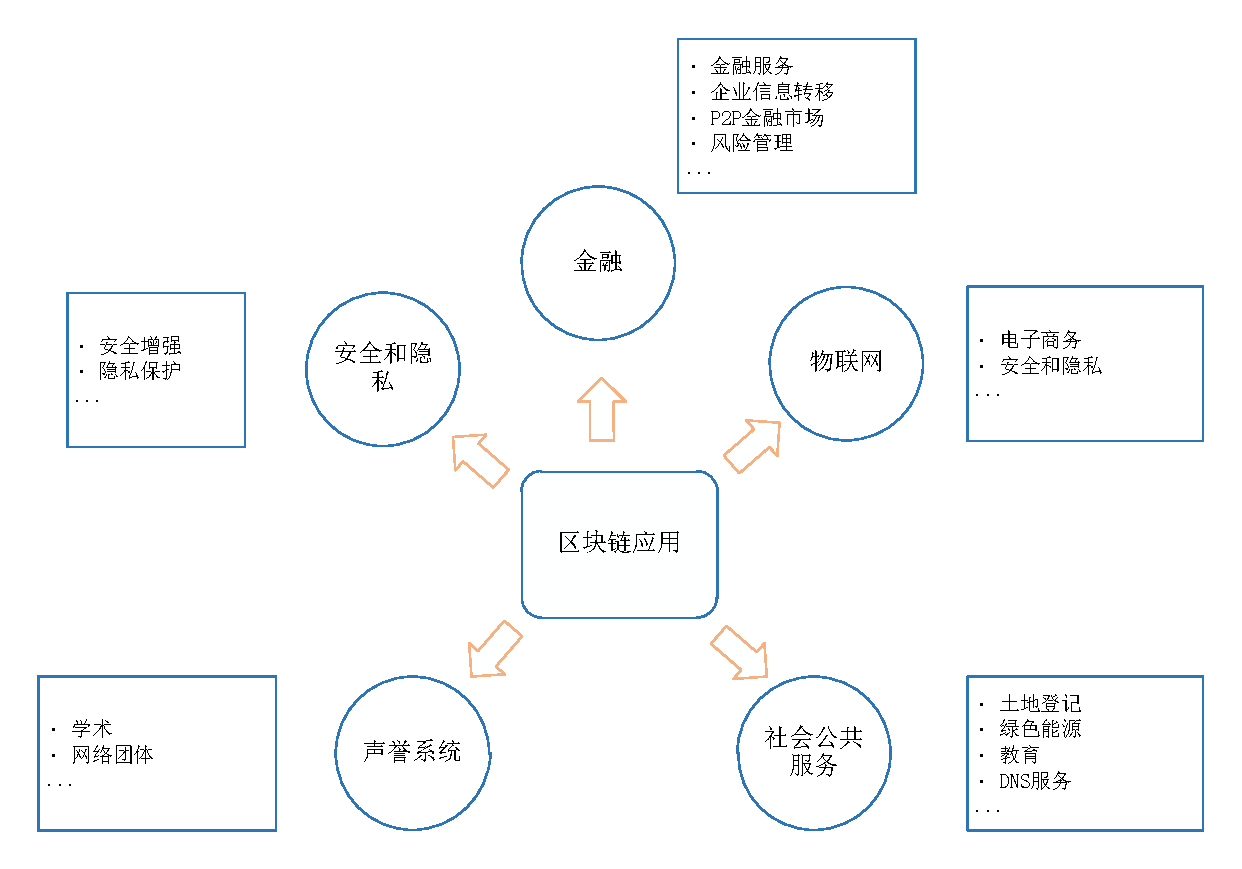
\includegraphics[width = 0.8\textwidth]{img/applications}
 	\caption{区块链典型的应用领域}\label{fig:applications}
\end{figure}

金融方面的应用包括金融服务、P2P金融市场、风险管理等,其中比特币、以太坊就是传统金融服务的另外一种表现形式,区块链给金融相关的应用带来了更好的特性;物联网方面的应用旨在使用区块链技术完成物联网实体之间数据的交换并提高自身的安全和隐私;与社会公共服务相关的区块链应用包括土地注册、绿色能源方面、教育和DNS服务等方面;名誉系统旨在利用区块链的不可篡改的特性,记录如学术论文或者网络团体的行为,提供有效的声誉证明。


% vim:ts=4:sw=4




















	% Copyright (c) 2014,2016 Casper Ti. Vector
% Public domain.

\chapter{PKI}

本章将对PKI系统进行详细介绍,首先从系统架构对PKI进行解析,阐述系统中包含的组成部分和各自的功能;其后将对证书进行介绍,包括证书的结构以及证书的生命周期;最后对本系统存在的问题以及相应的解决方案进行简要叙述。

\section{PKI系统}

公钥基础设施PKI(Public Key Infrastructure)作为一种遵循标准的密码管理平台,其可以为网络应用提供密钥和证书管理服务,使用户可以在多种应用环境下方便的使用加密和数字签名技术,从而保证数据的机密性、完整性、有效性和抗抵赖性。

本小节将从框架和其包含的相关组件对PKI进行介绍。

\subsection{PKI基本框架}

PKI框架中包括安全和操作策略,安全服务以及支持公钥密钥和证书管理的交互式协议。公钥和对应证书的生成、分发和管理将通过授权机构(CAs)、注册机构(RAs)和目录服务来完成\supercite{weise2001public},它们将会建立等级信任或者说信任链。以上提到CAs、RAs和目录服务可以将数字证书用于鉴定不同实体的身份,而PKI拥有如此架构的目的是为了能支持并完成数据、凭证在各种不安全环境下的安全交换。

\subsection{PKI的系统构成}

在PKI系统可能会包含一下组成部分:

\begin{itemize}
	\item 

	注册机构(RA)

	RA的作用是执行身份验证和处理新的数字证书请求、更新数字证书请求和吊销数字证书请求。

	\item

	授权机构(CA)

	CA将创建和发布数字证书以及证书吊销列表(CRLs),其颁发的数字证书将对主体名称(如用户表示)和绑定的公钥进行签名。

	\item

	验证结构(VA)

	VA是一个PKI的管理实体,可以用来检查数字证书的有效性。当证书的签发者和证书的状态管理服务有不同的服务提供者提供时,将使用到VA。

	\item

	用户

	PKI面对的用户是证书持有者或者密钥持有者,通过遵从认证运作规范(CPS)和证书策略(CP)获得证书,完成证书和密钥对的绑定。PKI系统中的用户可以是个体、组织或者非个人实体,有责任保存好自己的私钥不被泄露。

	\item

	依赖方

	依赖方在PKI系统中接收、验证和接受数字证书。

	\item

	证书策略(CP)

	证书策略是一组安全规则要求,适用于一类应用系统的共同安全需求。

	\item

	认证运作规范(CPS)

	CPS描述了CA提供数字证书服务的规则和处理方式,其中可能会包括提供服务描述,证书生命周期的管理细则、业务信息、法律义务和金融责任等。
\end{itemize}

图\ref{fig:pki}将给出以上所提到组件之间的关系,图中的剪头将表示数字证书和证书状态信息的传递。

\begin{figure}[htbp]
 	\centering
 	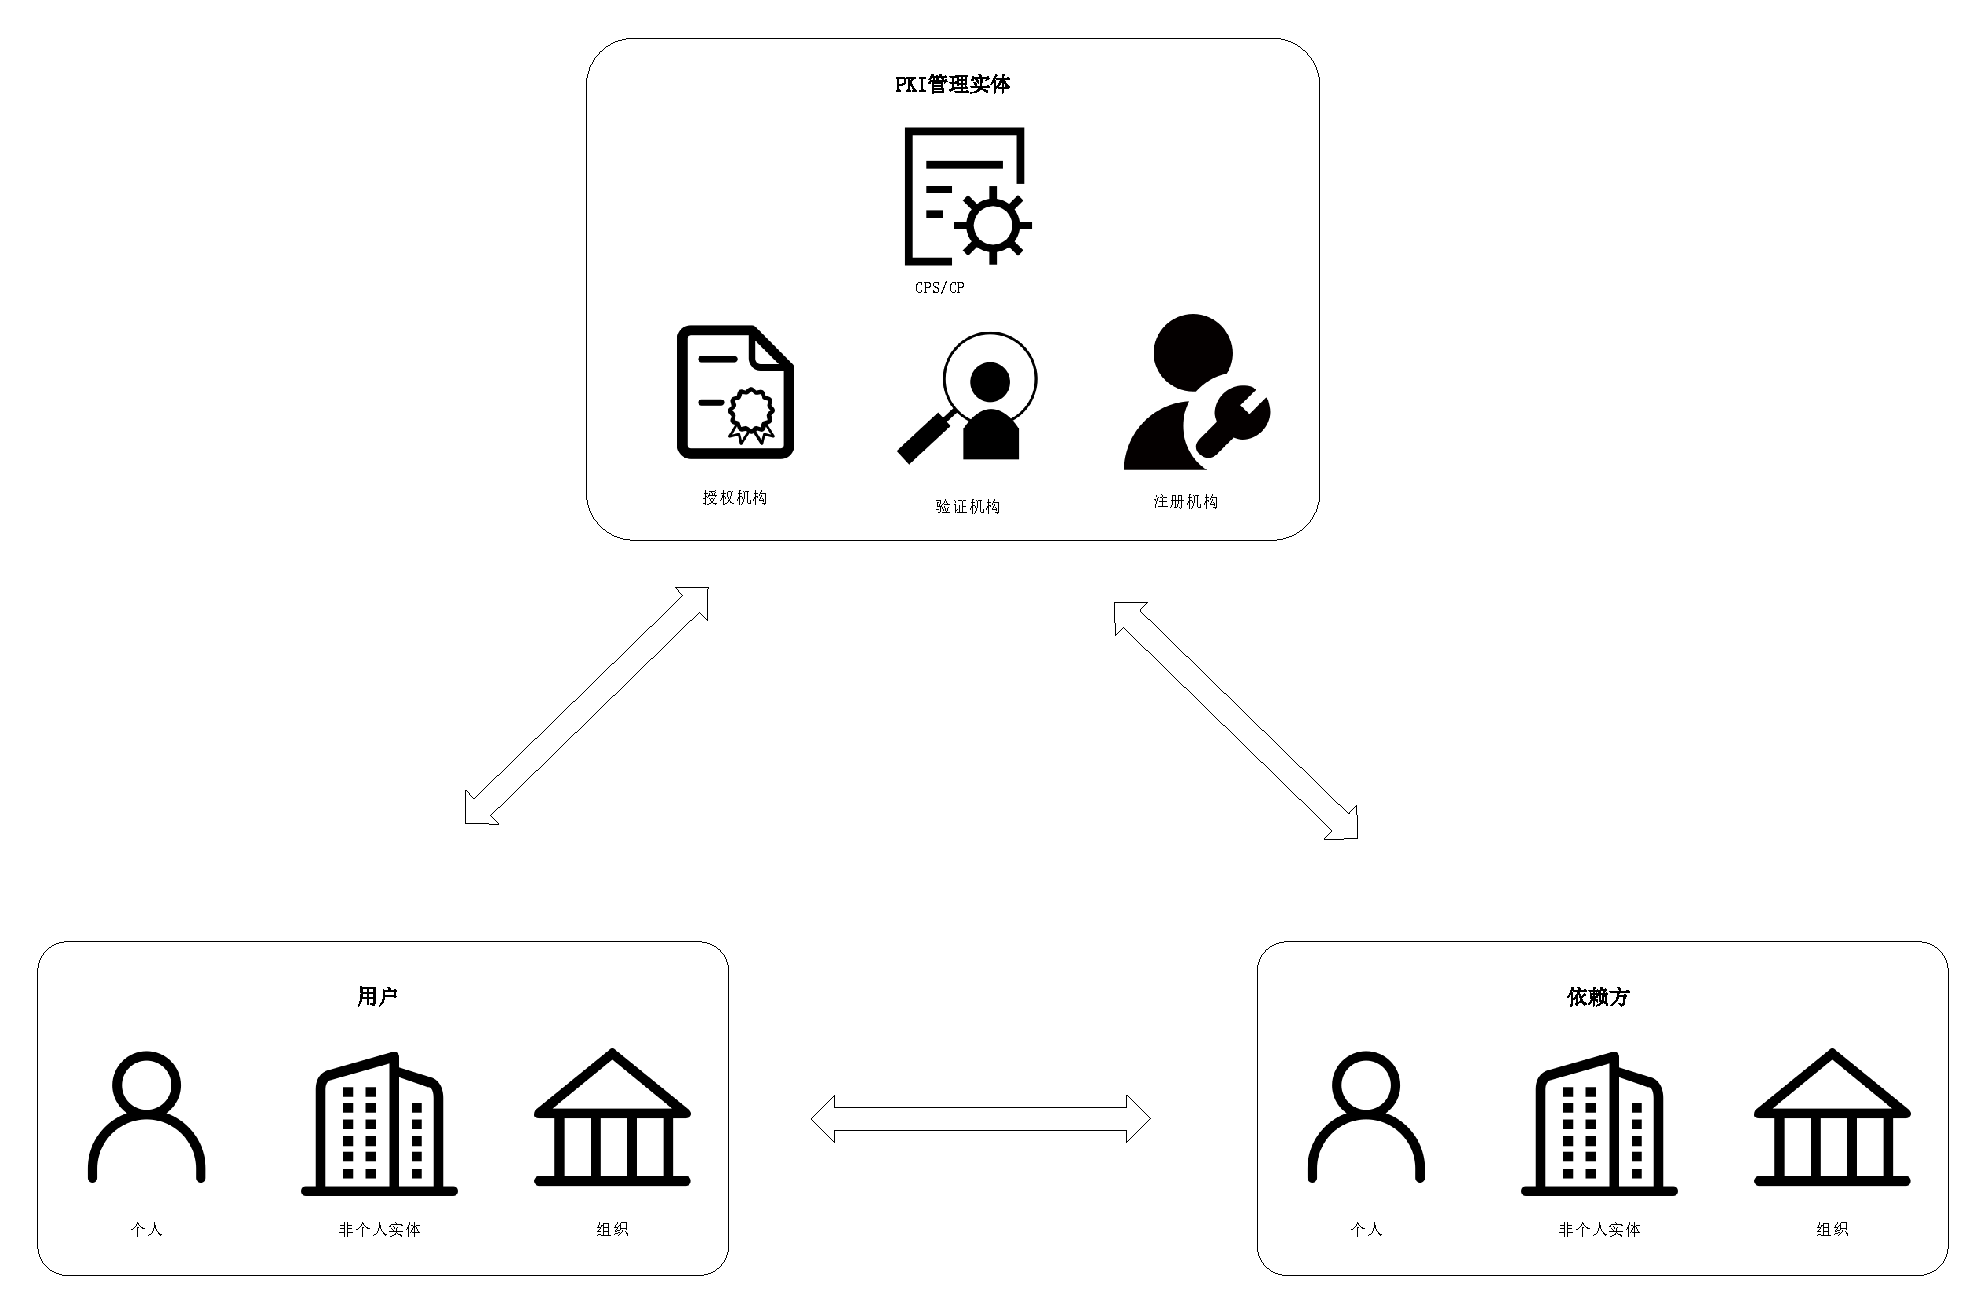
\includegraphics[width = 0.8\textwidth]{img/pki}
 	\caption{PKI组成部分}\label{fig:pki}
\end{figure}

\section{证书}

\subsection{证书的结构}

描述证书的结构。

\subsection{证书的生命周期}


证书作为包含公钥、数字签名以及一些其它附带信息的数字文档,在PKI系统中充当着公钥交换、存储和使用的介质。了解证书的申请、签发和使用,可以明白PKI系统的是如何运作,并从中发现可能存在的问题。

证书的声明周期从用户提交准备的证书签发请求(CSR)并提交给其选择的CA开始。CSR中包含了用户的公钥和相应的信息,并通过签名的方式表明对相应私钥的所有权。同时,CSR可以携带额外的信息元,但在实际使用过程中并没有全部使用。CA可以对CSR中的内容进行重写,放置一些其它的信息在证书中。

其后CA通过遵循验证流程,对用户进行身份验证。待成功完成验证之后,CA将签发证书,同时提供验证至根证书的所有中间证书。

得到证书后,用户就可在证书过期之前使用证书。如果证书对应的私钥泄露,证书将可以被吊销,该过程和证书签发的过程类似。

对于Internet PKI系统而言,根据以上证书流转流程,证书生命周期如图\ref{fig:cert_lifecycle}所示.

\begin{figure}[htbp]
 	\centering
 	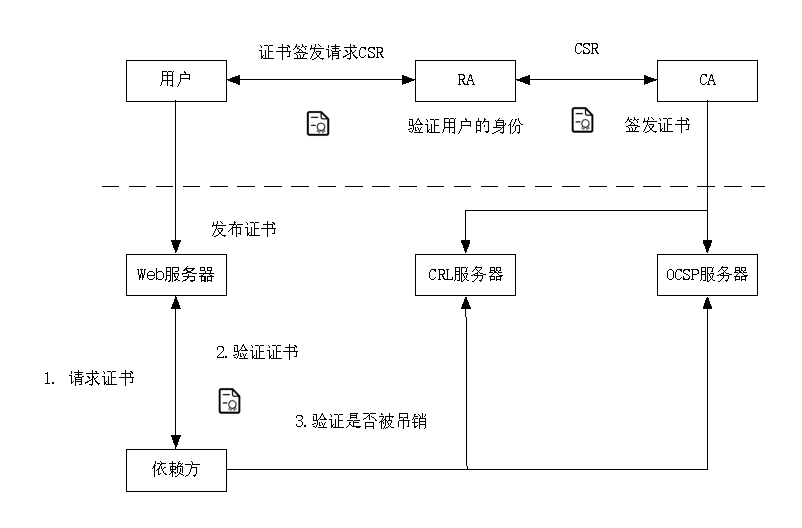
\includegraphics[width = 0.8\textwidth]{img/cert_lifecycle}
 	\caption{证书的生命周期}\label{fig:cert_lifecycle}
\end{figure}

\section{系统中存在的问题}

从安全的角度来看现有Internet PKI系统,其中存在着大大小小的各种问题,在本小节中,将对这些存在的问题进行简要概述。

当Web安全在1995年刚开始被谈及时,当时的互联网和现在是具有很大差异的,它的重要性并没有现在这么强。随着互联网的蓬勃发展,加密安全成为了商业中必备的一部分,关乎这一个企业的生死。现有的PKI系统和当初设计的目的是一致的,即为上电子商务操作提供足够的安全保障,更进一步可以说PKI系统希望提供商务安全。这种安全可以通较少的资金、更快的网页获取速度、可接受的不安全操作和不对用户做过多的限制来完成。本系统由CAs、寻利的商业实体和希望扩大市场份额的游览器供应商一起来组成。

CA在本系统中充当着信任的基础,其每年签发了数百万计的证书,这些证书将在互联网中流通并使用。虽然证书的安全性并没有想象中那么好,但是这个系统任然在正常的运转下去。同时,在那么不完美的情况下,用户还需要对申请的证书进行付费,然而并不是所有用户都愿意为之付出代价的,很简单的一个原因就是他们在付费之后希望得到完美的安全性保障。

在该系统中,存在着一下几个方面的问题:


\begin{itemize}
	\item

	域名权利过弱

	在PKI系统中最大的问题是任意CA在未经域名同意的情况下就可以对其签发证书,导致这个问题的主要原因是没有相关的技术策略去避免CA的疏漏和安全隐患,而该系统需要对CA给予相当高的信任。当CA数量比较少的时候,这个问题并没有那么严重,但是下周乃有数以百计的CA存在,很难保证每一个都不会存在行为过失或者不当的安全配置。一个系统的安全性取决于该系统最薄弱的环节,而PKI系统中存在着各种潜在的薄弱环节。所有的CA都需要被审计,但是审计的质量缺是不确定的。例如在2011年DigiNotar由于自身安全性问题就被黑客攻陷,最后导致自身倒闭。

	同时,另外一个存在的问题是CA是否可以被信任,它们能否在不需要监督的情况下为了公众的利益去做好自己的本质工作。这些被信任的CA可能在面对商业利益的时候放弃我们需要的安全。例如在2012年Trustwave承认其签发了低级别的假冒证书用于流量检查。虽然Trustwave是唯一公开承认自己做过类似事情的CA,大家相信这样的事情肯定大量存在。

	政府也可能会滥用PKI系统签发虚假证书,完成对任意域名的假冒。公众无法确保CA不会作为证书的前线,即使不是也无法保证这些CA不会被强迫的签发虚假证书。



	\item

	没有信任灵活度

	另外一个重要的问题是本系统缺乏信任的灵活度。依赖方将会存储一些列信任的根证书,一个CA只存在信任与否,并不存在中间地带。理论上,依赖方可以移除任何存储的CA,实际上这种情况只会在CA很小或者其已经被攻陷的时候发生。一旦一个CA签发了大量的证书,其将由于自身的大体量被不会被撤销。

	一些小的改善任然在被提出,例如对具有过失行为的CA不在信任打,是其之前的证书任然可以被使用。

	\item

	域名验证过于简单

	DV证书的签发是基于域名的WHOIS协议查询域名拥有者信息来完成的,也就是说大部分验证是通过邮件来完成的,而其本身的安全性就存在问题。如果域名被黑掉或者相应的邮箱密码被获取,那么就可以得到给域名的DV证书。同时通过拦截CA端验证信息也可以对发起攻击。



	\item 

	吊销不工作

	在一般情况下,对吊销证书的检查并没有那么严格,大多数情况都不能正常的工作。在2011年中有很多这样的例子,依赖方不得不将被泄露的证书通过特殊通信方式下载并存储在黑名单中,来保证吊销查询是可靠的。

	这样做的原因主要包括两个,首先将吊销信息发送各个系统需要一定的延时,在基准规则中允许CRL和OCSP的信息在10天是有效的,也就是说至少需要10天才能保证吊销信息被完全扩散出去;其次软失败机制在所有的游览器中被使用,当他们在查询吊销信息时会忽略掉所有失败的情况,一个主动的网络攻击者将可以轻易的拦截OCSP的请求,保证他们使用虚假的证书可以完美的被使用。

	由于以上的原因,Chrome开发者取消去证书吊销的检查,除非是EV类型的证书。对于重要的证书,例如中间证书,其间依赖于CRL信息的吊销通道查询相关内容。一种可能的解决方案是使用Must-stale的方案来保证证书的有效性。

\end{itemize}


\section{已有的改善措施}

为了解决X.509 PKI中的安全问题并削弱对CAs的信任,一系列的方案被提出来,本小节将对这些方案进行分类并简要叙述。



根据PKI中存在的主要三方实体域名、CA和客户端,可以对现有的方案进行分类,如图\ref{fig:Classification_of_PKI_proposals}所示。

\begin{figure}[htbp]
 	\centering
 	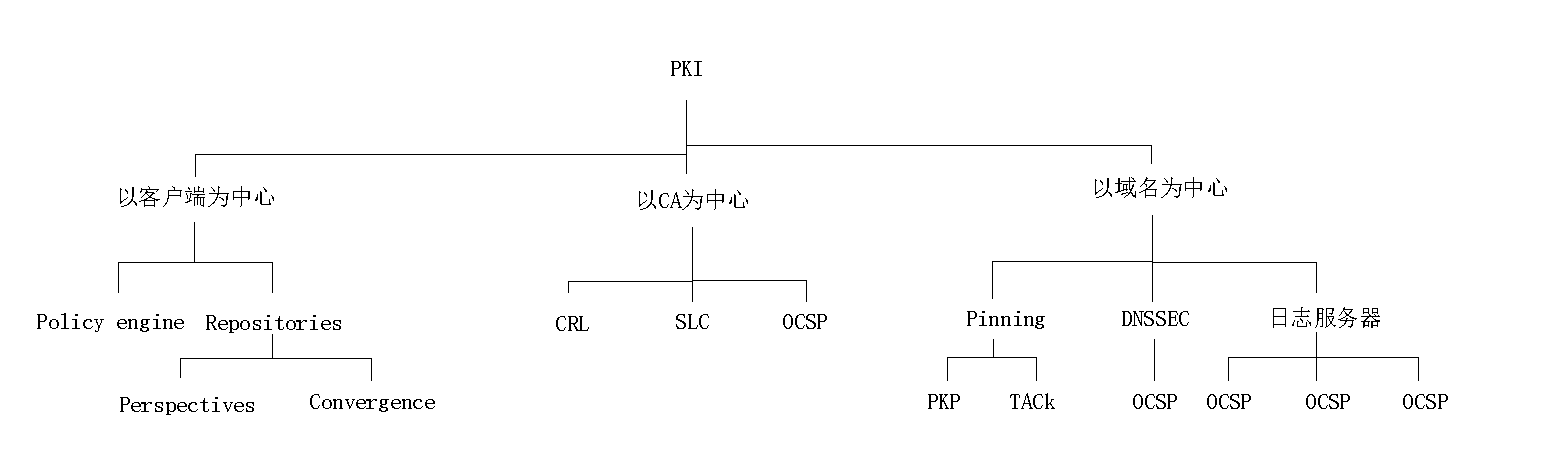
\includegraphics[width = 1.0\textwidth]{img/Classification_of_PKI_proposals}
 	\caption{PKI方案分类}\label{fig:Classification_of_PKI_proposals}
\end{figure}



\subsubsection{以客户端为中心的方案}

这类方案希望在客户端接受证书之前,可以更加准确的验证证书的有效性。Policy engine的方案允许客户端在本地制定信任决策,比如支持的密码算法,证书的一致性性等。

有一些其它的方案希望构建一个公共的域名证书存储厂库,使得客户端可以在接受到域名证书之后与厂库中的证书进行对比,确定证书的正确性,Perspectives 和 Convergence就输入这类方案。

以客户端为中心的方案并不需要对服务端进行的改动,但是其需要客户端建立额外的连接去查询资源厂库,这将在一定程度上降低建立HTTPS的速度。


\subsubsection{以CA为中心的方案}

X.509 PKI包含了证书吊销列表(CRL)标准,希望放置客户端与一个使用已经被吊销证书的域名之间发起建立TLS连接。但是这需要保证客户端需要能随时的访问到CRLs。为了进一步解决在线验证的问题,在线证书状态协议(OCSP)允许客户端通过CA的OCSP服务器去检查域名证书的状态。但是OCSP也拥有如安全、隐私、性能方案的顾虑。另外一个解决方案是短期证书(SLC),该方案希望签发短声明周期的证书,让域名定期的更换证书。SLC希望提带来和OCSP类似的好处,但是不需要在线验证。以证书为中心的方案严重依赖于游览器去检测和拉黑被攻陷CA签发的证书,这是这类方案的最大缺陷。


\subsubsection{以域名为中心的方案}


第三类方案允许域名拥有者积极控制和保护他们的证书而不被CA端的潜在问题所威胁。这些方案又可以分为以下三类:pining、DNSSEC、日志服务器。

1. Pinning-based(公钥固定)

如Public Key Pining(PKP)和Trust Assertions for Certificate Keys(TACK)等Pinning的方案希望域名宣称自己使用的密钥,以便客户端收到的密钥是否正确。但是这类方法有相应的安全缺陷,比如在第一次访问域名的时候无法给予安全保护。

2. DNSSEC-based

这类方案的全称叫基于DNS的命名实体鉴权(DANE),希望域名的所有者可以在DNSSEC实体上方式证书相关的特殊声明,例如可以为其签发证书的CA名单、声明接受的证书或者是声明验证证书有效性的节点,但是DANE的安全性严重的依赖于DNS操作的安全性行。


3. 日志服务器

另外一种使用比较多的方法是通过日志服务器的方案来记录CA的行为,为域名拥有者提供公共的、可审计的CA行为日志,监督CA的行为。例如 Sovereign Keys (SK)要求域名拥有者生成一个主密钥对来完成对TLS公钥的签名,并且将其主公钥以只读和只可追加的方式记录在时间服务器上。不行的是,SK需要客户端查询服务器,增加了延迟并牺牲了隐私。

证书透明(CT)的方案允许每个域名将自己的证书注册记录到一个公共日志服务器上,该服务器使用默克尔哈希树的结构来存储这些证书,并保证只能追加的性质。该服务器将返回一个不可否认的证书审计证明给域名,域名使用证书和该证明给客户端来完成TLS连接的建立。但是,本方案并不能防止当一个攻击者攻破了CA并创建并注册一个虚假的证书的情况,CT并不能阻止客户端接受这类证书。由于证书透明在设计过程中并没有强调证书的吊销,相应的证书吊销透明(RT)也被提出。为了提高CT对证书吊销的效率,证书签发吊销透明(CIRT)方案被提出。

另外一种基于日志服务器的方案称作可审计密钥设施(AKI),该方案希望保护域名和客户端遭受到单点失败攻击,比如某个CA的根密钥被泄露,通过制衡该系统中各个实体,AKI在保持高效处理证书操作的情况下,成功的将信任分散到了多个实体,并可以检测出实体的恶意行为。




% vim:ts=4:sw=4


























































	% Copyright (c) 2014,2016 Casper Ti. Vector
% Public domain.

\chapter{基于区块链的命名实体鉴权方案设计与实现}

本章节将阐述基于区块链的命名实体鉴权方案,首先从系统设计的整体架构出发,描述本系统中包含的系统角色和架构;然后对鉴权方案进行详细阐述,并理论论证鉴权方案的有效性和可靠性;最后对模块实现的进行阐述。


\section{系统设计}

本部分将从系统涉及的角色和模块对本系统的整体架构进行描述。

\subsection{系统角色}

针对证书申请和使用流程,在PKI系统中涉及的角色包含以下三类:
\begin{itemize}
	\item 证书授权者(CA):在PKI系统充当证书签发和管理的角色。
	\item 证书申请者:证书申请者在PKI系统中作为证书的持有者,在初始过程中需要向CA提出证书申请,在完成身份验证之后即可获得相应的证书,并在使用过程中提供证书以证明自己的身份,在本场景中,证书的申请者指域名或者站点。
	\item 证书验证cd者:证书验证者是证书的受用者,在通信过程中需要认证对方身份的时候,获得证书并完成有效性验证。
\end{itemize}

不同的角色在PKI证书的流转过程中对证书的控制权不尽相同,证书授权者作为证书的签发方,对其是否签发证书具有绝对的主动权,甚至可以在未经证书申请者同意的情况下签发恶意证书;证书申请者则只能发起证书申请,不能对证书是否被签发起到决定权;证书验证者则只能验证证书是否合法,对于恶意CA私自签发的虚假证书,并没有辨别真伪的能力。

可以看出,在传统的PKI系统中,证书申请者和证书授权者之间的地位是不对等的,这是由于证书授权方对证书的拥有绝对管理权,所以在PKI系统中,需要所有的角色对中心化的CA绝对性信任。为了使得证书申请者和证书授权者之间的权利更加均衡,需要提高证书申请方对证书签发的控制权,使用本文中涉及的命名实体鉴权方案,保证未被允许签发的证书签发机构无法对证书进行私自签发。

在本方案中,以上提到的三类角色具有以下特性:
\begin{itemize}
	\item 证书授权者(CA):在本方案中,其角色和功能保持不变,负责对发起证书申请的实体进行证书颁发。
	\item 证书申请者:在本方案中,其将利用区块链完成身份的认证,并将自己信任的CA列表发布在区块链上。
	\item 证书验证者:在本方案中,验证者可以通过区块链查询身份确认实体的信任CA列表,保证证书的签发是合法的。
	\item 验证节点:在本方案中,验证节点作为证书申请者的身份验证者,通过这些节点完成对区块链上证书申请者的身份认证。
\end{itemize}

\subsection{系统架构}

本系统依托于现有的PKI体系,并基于区块链作为存储平台,在其上进行证书申请者信任CA列表的存储,系统中的各个角色都要通过本系统中的区块链进行数据交流。更为重要的是,域名站点需要在此基础上进行身份认证,作为信任建立的根基。系统的总体设计如图\ref{fig:test}所示:


\begin{figure}[htbp]
 	\centering
 	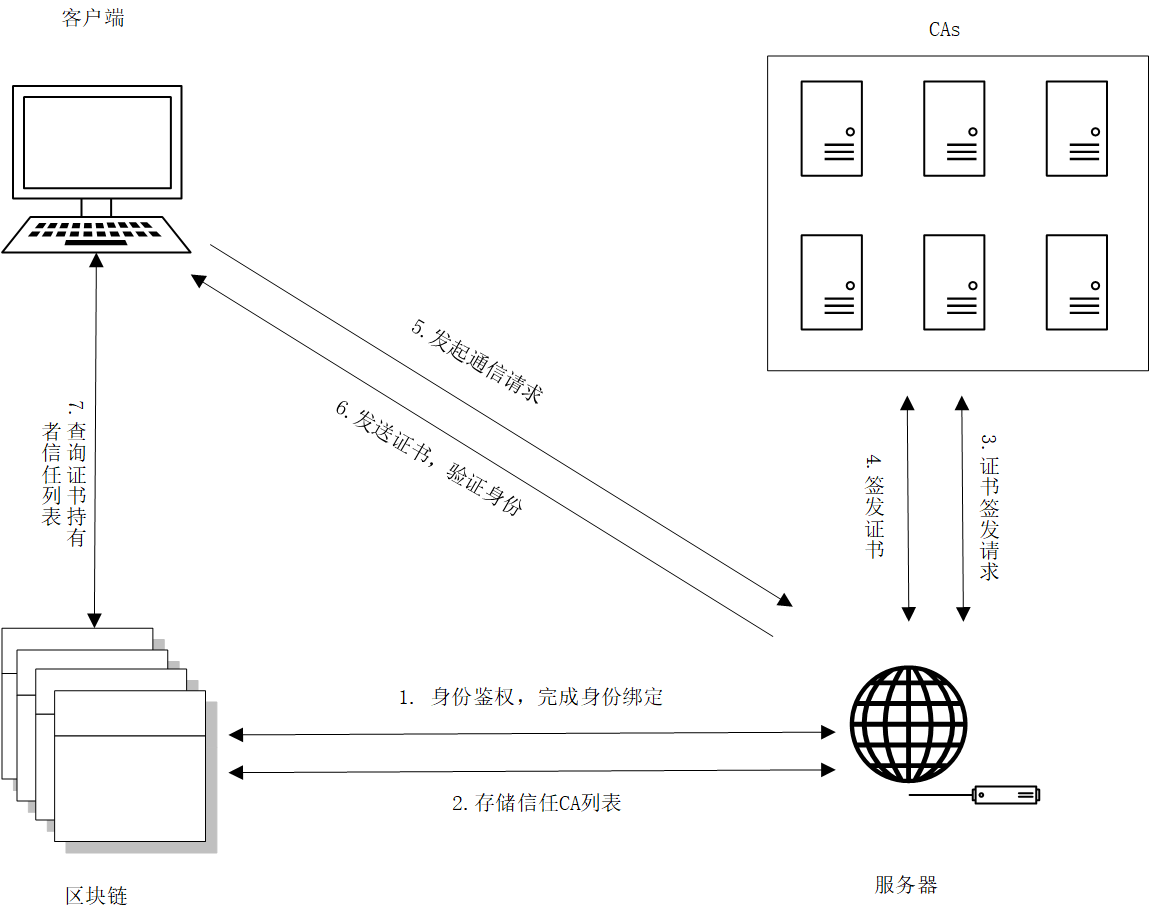
\includegraphics[width = 0.8\textwidth]{img/art}
 	\caption{总体架构}\label{fig:test}
\end{figure}


在本系统中,域名站点作为证书申请者,向区块链发起身份认证请求,当交易被记录到区块链上之后,域名站点根据交易提供验证信息,供验证节点对其身份进行验证;完成验证之后,域名即可将自己信任的CA列表发布到区块链上,并向自己信任的CA进行证书申请;完成申请后,即可将证书用在与用户通信的过程中,进行身份证明,此时证书验证者将通过区块链进行信任列表查询,判断该证书是否是合理签发的。



\section{身份绑定方案}

在本方案中,域名需要将自己信任的CA列表记录到区块链上,但是区块链具有去中心化和匿名特性的底层技术,域名直接将自己的信任CA放置到区块链上是不具有可信性的,之前需要完成区块链地址(或者公钥)和域名本身的绑定,完成地址与域名之间的实体认证。本文将提供基于验证时间和基于验证次数的身份绑定方案。

身份绑定过程大致分为3个步骤:

\begin{enumerate}
	\item 域名发送认证请求到区块链上;
	\item 待交易确认后,根据交易和区块在服务端放置验证;
	\item 验证节点对其进行验证,达到验证期限或者次数后,完成身份绑定。
\end{enumerate}

\subsection{基于验证时间的身份绑定方案}

基于验证时间的方案旨在让绑定者提供验证信息持续一段时间,以供所有节点对其进行验证,当提供的验证达到指定时间后,即认为其对该域名服务器的所有权,完成指定地址和域名的绑定。

\noindent\textbf{假设}

假设绑定者A拥有公钥$Pk_A$,私钥$Sk_A$以及域名$example.com$,其需要完成$(Pk_A, example.com)$的绑定;某一验证者B拥有公钥$Pk_B$和私钥$Sk_B$。

\noindent\textbf{交易类型}

在本方案中,包含以下两种类型的交易:

\begin{enumerate}
	\item 绑定请求交易$Tx_{req}$:交易请求者发布绑定请求,包含了自己的公钥$Pk_A$和域名$examle.com$。
	\item 检举交易$Tx_{rep}$:验证节点发现绑定者的验证信息放置不准确,可以提出检举交易,驳回身份绑定。
\end{enumerate}

\noindent\textbf{流程}

绑定的具体流程包含以下四步:

\begin{enumerate}
	\item $A$发布绑定交易$Tx_{req}(Pk_A, example.com)$到区块链上;
	\item 根据需要的绑定信息$(Pk_A, example.com)$,计算$(Path, Chal) = F(Pk_A, example.com)$放置在自己控制的域名下,即访问$example.com/Path$即可获取到$Vcode = Sign_{Sk_A}(Chal)$值;
	\item 验证者$B$访问域名验证A是否正确操作,如果不,发送检举交易$Tx_{rep}(Pk_A, example.com)$到区块链;
	\item $A$保持验证时长$T$后,可停止该验证服务,完成绑定。
\end{enumerate}

在该绑定过程中,首先需要绑定者将绑定信息自己的$Pk_A$和自己的域名$example.com$发布到区块链上,将绑定身份信息展现给所有的验证节点,并根据函数$F$生成相关验证内容。我们选择哈希函数$sha256$作为函数原型,将$Pk_A$和$example.com$直接拼接后作为输入,将计算得到的256位哈希值前128位赋值给$Path$、后128位赋值给$Chal$:

\begin{equation}\label{eqF}
Path_{128}||Chal_{128} = sha256(Pk_A||example.com)
\end{equation}

\begin{equation}\label{eqSign}
Vcode = Sign_{Sk_A}(Chal)
\end{equation}

绑定者将以上得到的$Vcode$值放置在网站的$example.com/Path$目录下,作为身份验证的内容,供所有验证节点验证。如果验证节点在验证过程中发现其并没有正确的放置验证信息,将可以通过发送检举信息$Tx_{rep}$对身份绑定消息进行驳回。


\subsection{基于验证次数的身份绑定方案}

基于验证次数的方案需要在绑定者发布绑定信息后,选择出合适的验证者,对绑定者的验证信息进行确认,当验证的次数达到规定次数后即可完成省份绑定。

\noindent\textbf{假设}

假设绑定者A拥有公钥$Pk_A$,私钥$Sk_A$以及域名$example.com$,其需要完成$(Pk_A, example.com)$的绑定;某一验证者B拥有公钥$Pk_B$和私钥$Sk_B$。

\noindent\textbf{交易类型}

在本方案由于需要特定验证者完成验证信息的确认,相比于基于时间的验证方案,增加了验证交易类型,包含一下三类交易类型:

\begin{enumerate}
	\item 绑定请求交易$Tx_{req}$:交易请求者发布绑定请求,包含了自己的公钥$Pk_A$和域名$examle.com$。
	\item 检举交易$Tx_{rep}$:验证节点发现绑定者的验证信息放置不准确,可以提出检举交易,驳回身份绑定。
	\item 验证交易$Tx_{vfy}$:验证者在完成验证信息的对比后,在验证通过的情况下发送验证通过的交易。
\end{enumerate}

\noindent\textbf{流程}

基于验证次数的身份绑定方案相比于基于验证时间的方案需要验证者更多的和区块链进行交互,在验证过程中需要将验证是否通过的信息提交到区块链上去,具体流程如下:

\begin{enumerate}
	\item $A$发布绑定交易$Tx_{req}(Pk_A, example.com)$到区块链上;
	\item  A获取$Tx_{req}$所在位置区块信息$Info_{block}$,并根据其计算值$(Path, Chal) = F(Info_{block})$放置在自己控制的域名下,及访问$example.com/Path$即可获取到$Vcode = Sign_{Sk_A}(Chal)$值;
	\item 根据交易$Tx_{req}$计算符合该条请求的验证者:${v_1, v_2, ... , v_k}$,假设$B$为其中一个验证者
	\item B从$example.com/Path$获取验证内容,提交交易$Tx_{vfy}(Pk_B, Pk_A, C)$ 完成验证。
	\item 在经过$K$个验证过后,即完成绑定。
\end{enumerate}

整体流程和基于时间的方案类似,需要绑定者将自己的公钥$Pk_A$和自己的域名$example.com$发布到区块链上,然后通过公式函数获得\eqref{eqF}和\eqref{eqSign}计算得到$Path$和$Vcode$的值放置到自己的服务器上;验证者通过\eqref{eqF}计算获得$Path$、$Chal$和$Pk_A$对验证信息进行确认,确认通过后发送验证交易$Tx_{vry}$到区块链上完成一次验证,待达到验证次数$K$后,即完成身份绑定。

\noindent\textbf{验证者的选取}

在本方案中,需要合理的选取验证者,避免节点为了保证自己的利益,将其他节点的验证交易滞后提交到区块链中的情况;另外一方面,如果验证节点不是经过筛选,而是每个节点都可以对绑定身份进行验证的话,恶意的绑定者可以使用不同的公钥作为验证节点,然后对恶意绑定进行确认;同时,正常的验证者为了获得更多的奖励,也会申请尽量多的账户对交易进行验证,从中获得更多的获益。

为了避免以上的情况出现,本方案中设计了依据绑定信息随机选择验证节点的方法,保证验证可以安全有效的进行。当绑定信息被发布到区块链上后,根据绑定信息$Pk_A$和$example.com$,将其装换为基准公钥$Pk_{cmp}$:

\begin{equation}\label{eqGenCmpPk}
Pk_{cmp} = sha-512(Pk_A||example.com)
\end{equation}

在得到基准公钥后,验证节点计算公钥$Pk_v$与基准公钥$Pk_{cmp}$之间的海明距离,如果其距离小于某一个值$d$,就具有验证该次绑定的权力,可以向区块链提交验证结果。为使得能够有住够多的验证者,让身份绑定过程可以更加高效的进行,随着时间的推移,对海明距离的约束$d$将会逐渐变大。

[需要展开一下]




\subsection{奖励惩罚机制}

为了促使本方案有足够多的验证节点加入,保证身份绑定能够完整有效的进行,需要对验证节点给予一定的奖励。在验证过程中,如果发现存在未合理放置验证信息的 域名,将可以发起检举交易到区块链上,待交易确认后,其可以得到相应的奖励;为保证本系统中的奖励平衡,发起绑定者需要付出一定的代价,而验证者发现错误时,将 可以获取得到相应的奖励。所以涉及到的奖励和惩罚机制包括以下三点:

\begin{itemize}
	\item 在发起绑定交易时,绑定者需要付出一定的代价
	\item 在完成验证之后,验证者将会获得相应的奖励(仅在基于验证次数的方案中使用)
	\item 在发现非法绑定时,验证者将可以发起交易获得相应奖励
\end{itemize}

如上所述,后两条为奖励机制,其目的是吸引更多的人加入到本系统之中,使得身份绑定可以顺利的完成,并具有较高的真实性;而第一条规则的设计让身份绑定者需要付出代价,而不是无限制的随意的在本方案中发起身份绑定操作,从而避免了恶意的破坏者无限度的去发起无效的身份绑定,从而影响本系统中正常身份绑定者的顺利进行。同时,由于验证者在完成验证或者发现验证不通过的时候,将会获得奖励,而这些奖励不是凭空产生的,而是绑定者所付出的相应费用。


\subsection{安全性分析}

\subsubsection{站点对域名服务器的控制权}

为了保证绑定者对域名服务器拥有控制权,在以上方案中,使用提交的$Tx_{req}$来生成验证内容$Path$和$Chal$,保证了验证内容和提交请求的相关性;同时在\eqref{eqF}中使用$sha256$作为随机函数,将提交内容转换为验证内容,该过程是一个不可逆的过程,从验证内容到提交内容的生成是很难完成的,保证了很难通过验证内容去构造提交内容。在放置的验证内容中,$Vcode$是使用绑定公钥对应私钥对$Chal$进行签名得到的,保证了绑定者对私钥的拥有权。


\subsubsection{验证交易真实有效}

基于时间的验证方案中不需要提交者发起验证提交,在发现错误的时候菜需要发送检举交易;对于基于验证次数的方案而言,需要提交验证内容即$Vcode$,因为有签名的存在,验证节点不能凭空的发送验证交易,需要通过服务器提供的验证信息才能正确的完成验证。

绑定者如果未能正确的放置验证内容,或者通过其它方式公布验证内容,导致验证过程依旧执行,那么其他验证节点可以通过检举交易对其发起检举。


\subsubsection{验证时间的选择}

在区块链上有确认交易的概念,以保证交易被正确的收录到了区块链中,并在很大程度上达到不可篡改的安全级别\supercite{nakamoto2008bitcoin}。假设区块链上的交易确认块数为$\Delta$,出块的平均时间为$T_{avg}$,在一个$\Delta*T_{avg}$的时间之后,交易将被确认有效,在此期间,所有的节点都可以对该条交易的验证内容进行确认,一旦发现不符合的现象,即可发起检举交易,完成检举。

\subsubsection{验证次数的选择}




\section{模块实现}

本文以以太坊为例作为区块链底层架构,利用其智能合约完成以上方案的逻辑实现,PKI各个实体通过与智能合约之间交互,存储并获取相关数据,完成对信任CA列表的读写,并最终完成对证书有效性的进一步确认。

根据上面的设计,以以太坊作为区块链基础,本系统如\ref{fig:module}图分为四个模块进行实现:智能合约、域名客户端、验证节点客户端、游览器验证插件。

\begin{figure}[htbp]
 	\centering
 	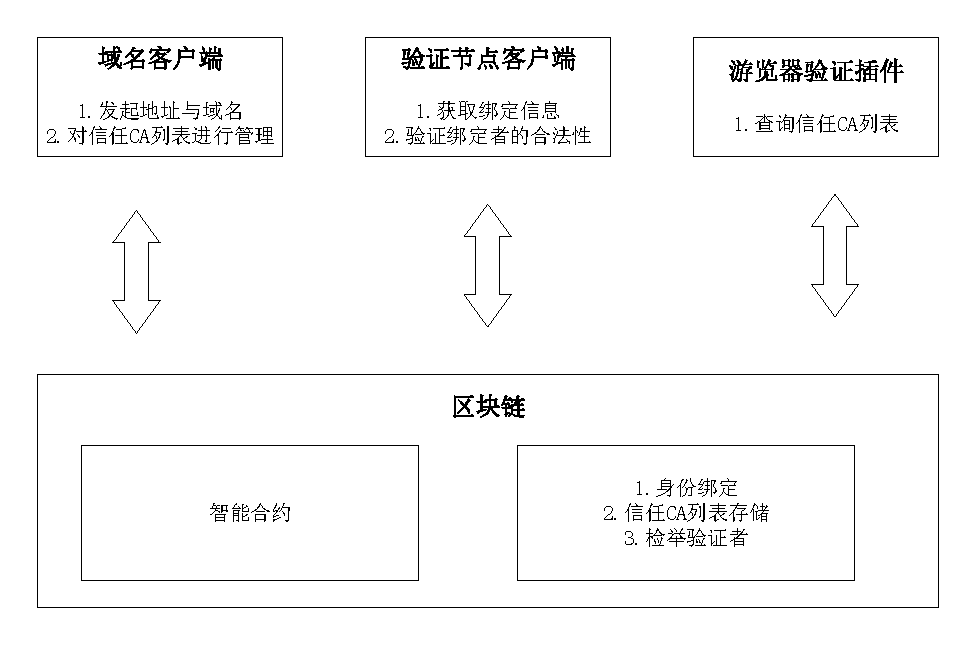
\includegraphics[width = 0.8\textwidth]{img/module}
 	\caption{系统模块}\label{fig:module}
\end{figure}

\subsection{智能合约}

智能合约作为可以在区块链上实现其他逻辑操作的一种工具,在本部分,将给予以太坊作为底层区块链基础,在其上开发具有本文所述方案的智能合约,提供其它模块访问区块链的相关接口和功能,完成本文所述方案中的逻辑操作。

在智能合约中需要提供身份绑定接口、信任列表修改接口、信任列表存储接口以及检举接口。

\subsubsection{身份绑定接口}

身份绑定接口主要提供给域名客户端和验证节点客户端使用,针对不同的客户端有两种不同的的操作:身份绑定请求和身份绑定确认。

身份绑定请求操作是由域名通过域名客户端发起,发送需要绑定的域名和公钥到智能合约中进行登记,并放置合法的验证内容到自己的服务器上,供验证节点对其进行验证。

在身份绑定请求发送成功之后,验证节点客户端可以获得最新的待验证身份绑定信息,并对身份绑定的信息进行验证,如果验证通过,则会通过智能合约调用身份绑定确认操作,完成身份绑定验证。

\subsubsection{信任列表修改接口}

域名在完成身份绑定之后,即拥有了与域名相关联的公私钥对,通过对公钥对应内容的控制调整自己信任的CA列表。其通过调用信任CA列表对信任CA进行修改操作,并存储在区块链上供其它人查阅。


\subsubsection{检举接口}

当验证者发现带确认的域名并未正确放置验证内容时,即可调用检举接口,完成对公钥对本次域名绑定的检举。

\subsection{域名客户端}

域名作为证书的申请者,需要将自己的可信任CA列表存储到区块链上,以供证书受用者在使用证书的过程中对证书的真伪进行进一步检查。

域名客户端需要与区块链进行交互,实现域名和公钥的绑定以及对自己可信CA列表的控制,主要包括以下操作:

\begin{itemize}
	\item 

	发起身份绑定请求

	通过调用智能合约身份绑定接口,发送需要绑定的域名和公钥,完成身份绑定请求操作。

	\item 

	修改信任CA列表

	在完成身份绑定之后,域名客户端将可以控制公钥和域名所对应的信任CA列表,通过调用智能合约中的信任列表修改接口,完成对自身信任CA列表的管控。


\end{itemize}

\subsection{验证节点客户端}

验证节点是本系统中身份鉴权的重要组成部分,是身份绑定有效性的保证,只有住够多验证节点存在的情况下,才可以保证身份确认的有效。

验证节点的主要工作是实时的查询验证请求并对验证请求进行验证,并根据其验证请求计算自己是否符合验证节点的要求,如果符合的话将进行验证确认操作,如果不是,也可以进行验证,对不符的验证提交检举交易。


\subsection{游览器验证插件}


游览器Web PKI中证书受用者的客户端,在原有体系结构中充当着检查证书真伪的角色。在本方案中,为了保证被恶意CA私自签发的证书可以被识别出来,需要在客户端进行对证书进行额外的检查,也就是需要游览器需要有区块链进行交互,查询收到的证书是否由证书申请者信任的CA所签发。


% vim:ts=4:sw=4

	% Copyright (c) 2014,2016 Casper Ti. Vector
% Public domain.

\chapter{基于区块链的命名实体鉴权系统实现}



% vim:ts=4:sw=4

	% 结论。
	% Copyright (c) 2014,2016 Casper Ti. Vector
% Public domain.

\specialchap{结论}
\pkuthssffaq % 中文测试文字。

% vim:ts=4:sw=4


	% 正文中的附录部分。
	\appendix
	% 排版参考文献列表。bibintoc 选项使“参考文献”出现在目录中;
	% 如果同时要使参考文献列表参与章节编号,可将“bibintoc”改为“bibnumbered”。
	\printbibliography[heading = bibintoc]
	% 各附录。
	% Copyright (c) 2014,2016 Casper Ti. Vector
% Public domain.

\chapter{附件}
\pkuthssffaq % 中文测试文字。

% vim:ts=4:sw=4


	% 以下为正文之后的部分,默认不进行章节编号。
	\backmatter
	% 致谢。
	% Copyright (c) 2014,2016 Casper Ti. Vector
% Public domain.

\chapter{致谢}

转眼间三年的硕士时间即将过去,在这里首先要特别感谢关志老师在这三年中对我的指导和关怀。关老师是一位在信息安全和密码领域知识渊博的学者,带领我去学习和了解专业相关的知识,并教我如何去研究并解决问题。感谢关老师在我研究生学习上和毕业论文上的耐心指导,以及平时对我们在生活上的关心和照顾。同时也要感谢陈钟老师在研究生其间对我的指导和帮助,感谢实验室其他老师在这三年中给我的教导。

感谢Abba与我在区块链方面的学习和交流,感谢刘超、王珂、李悦在毕业论文书写其间的讨论和建议;也感谢赵晓濛在三年研究生工作和学习中的帮助,感谢苏超、赖蔚两位师弟在实验室工作中的协助;感谢已经毕业的王康达、刘洪元、王诗吟、董秋香等师兄师姐在研究生学习和生活中的帮助,感谢三位室友李奕、邱兆鹏、林武桃三年的帮助和陪伴,也感谢马凌霄、董自鸣等大学同学的陪伴。

最后感谢我的父母和家人,在生活和学习中始终给予我帮助和支持,是我不断前进的力量源泉。

在此论文完成之际,谨向三年研究生学习生活中给予我关心和帮助的良师益友及亲人们致以最诚挚的谢意!





% vim:ts=4:sw=4

	% 原创性声明和使用授权说明。
	% Copyright (c) 2008-2009 solvethis
% Copyright (c) 2010-2017 Casper Ti. Vector
% All rights reserved.
%
% Redistribution and use in source and binary forms, with or without
% modification, are permitted provided that the following conditions are
% met:
%
% * Redistributions of source code must retain the above copyright notice,
%   this list of conditions and the following disclaimer.
% * Redistributions in binary form must reproduce the above copyright
%   notice, this list of conditions and the following disclaimer in the
%   documentation and/or other materials provided with the distribution.
% * Neither the name of Peking University nor the names of its contributors
%   may be used to endorse or promote products derived from this software
%   without specific prior written permission.
%
% THIS SOFTWARE IS PROVIDED BY THE COPYRIGHT HOLDERS AND CONTRIBUTORS "AS
% IS" AND ANY EXPRESS OR IMPLIED WARRANTIES, INCLUDING, BUT NOT LIMITED TO,
% THE IMPLIED WARRANTIES OF MERCHANTABILITY AND FITNESS FOR A PARTICULAR
% PURPOSE ARE DISCLAIMED. IN NO EVENT SHALL THE COPYRIGHT HOLDER OR
% CONTRIBUTORS BE LIABLE FOR ANY DIRECT, INDIRECT, INCIDENTAL, SPECIAL,
% EXEMPLARY, OR CONSEQUENTIAL DAMAGES (INCLUDING, BUT NOT LIMITED TO,
% PROCUREMENT OF SUBSTITUTE GOODS OR SERVICES; LOSS OF USE, DATA, OR
% PROFITS; OR BUSINESS INTERRUPTION) HOWEVER CAUSED AND ON ANY THEORY OF
% LIABILITY, WHETHER IN CONTRACT, STRICT LIABILITY, OR TORT (INCLUDING
% NEGLIGENCE OR OTHERWISE) ARISING IN ANY WAY OUT OF THE USE OF THIS
% SOFTWARE, EVEN IF ADVISED OF THE POSSIBILITY OF SUCH DAMAGE.

{
	\ctexset{section = {
		format+ = {\centering}, beforeskip = {40bp}, afterskip = {15bp}
	}}

	% 学校书面要求本页面不要页码,但在给出的 Word 模版中又有页码且编入了目录。
	% 此处以 Word 模版为实际标准进行设定。
	\specialchap{北京大学学位论文原创性声明和使用授权说明}
	\mbox{}\vspace*{-3em}
	\section*{原创性声明}

	本人郑重声明:
	所呈交的学位论文,是本人在导师的指导下,独立进行研究工作所取得的成果。
	除文中已经注明引用的内容外,
	本论文不含任何其他个人或集体已经发表或撰写过的作品或成果。
	对本文的研究做出重要贡献的个人和集体,均已在文中以明确方式标明。
	本声明的法律结果由本人承担。
	\vskip 1em
	\rightline{%
		论文作者签名:\hspace{5em}%
		日期:\hspace{2em}年\hspace{2em}月\hspace{2em}日%
	}

	\section*{%
		学位论文使用授权说明\\[-0.33em]
		\textmd{\zihao{5}(必须装订在提交学校图书馆的印刷本)}%
	}

	本人完全了解北京大学关于收集、保存、使用学位论文的规定,即:
	\begin{itemize}
		\item 按照学校要求提交学位论文的印刷本和电子版本;
		\item 学校有权保存学位论文的印刷本和电子版,
			并提供目录检索与阅览服务,在校园网上提供服务;
		\item 学校可以采用影印、缩印、数字化或其它复制手段保存论文;
		\item 因某种特殊原因需要延迟发布学位论文电子版,
			授权学校在 $\Box$\nobreakspace{}一年 /
			$\Box$\nobreakspace{}两年 /
			$\Box$\nobreakspace{}三年以后在校园网上全文发布。
	\end{itemize}
	\centerline{(保密论文在解密后遵守此规定)}
	\vskip 1em
	\rightline{%
		论文作者签名:\hspace{5em}导师签名:\hspace{5em}%
		日期:\hspace{2em}年\hspace{2em}月\hspace{2em}日%
	}

	% 若需排版二维码,请将二维码图片重命名为“barcode”,
	% 转为合适的图片格式,并放在当前目录下,然后去掉下面 2 行的注释。
	%\vfill\noindent
	%\includegraphics[height = 5em]{barcode}
}

% vim:ts=4:sw=4

\end{document}

% vim:ts=4:sw=4
